\chapter{Per-Run Convergence Curves}
\label{app:curves}

This appendix gathers the per-run validation curves and the
best-loss summary for the runs of Chapter~\ref{ch:experiments}.
The summary table is reproduced verbatim from the run-log
artefact \texttt{thesis/assets/figures/ablation\_summary.txt};
the curves are emitted by
\texttt{scripts/thesis\_figs/val\_curves.py}.

\section{Mask-policy ablation curves (E12--E15)}
\label{app:curves-mask}

\begin{figure}[htbp]
\centering
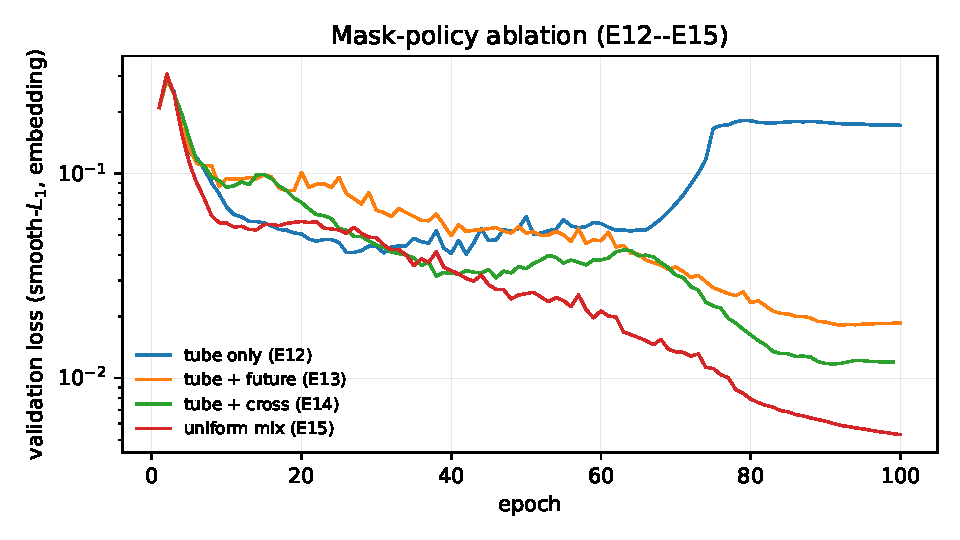
\includegraphics[width=0.95\linewidth]{assets/figures/curves_mask_policy.pdf}
\caption{Validation smooth-$L_{1}$ versus epoch for the four
mask-policy mixtures. The tube-only arm (E12) shows the
post-curriculum divergence of Finding~F3; the uniform mix (E15)
is monotone to epoch~99 and sets the sanity floor of
Finding~F11.}
\label{fig:curves-mask-app}
\end{figure}
\FloatBarrier

\section{EMA decay sweep curves (E17--E20)}
\label{app:curves-ema}

\begin{figure}[htbp]
\centering
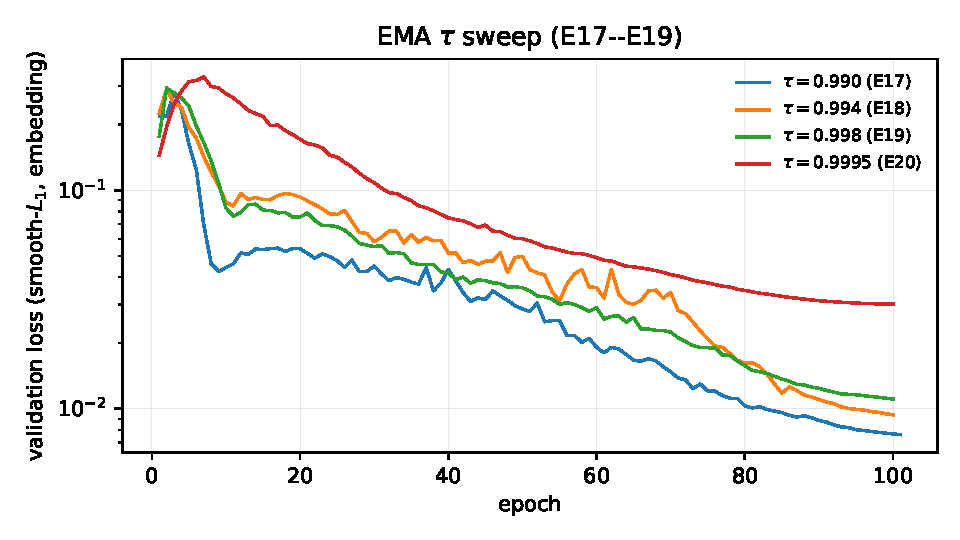
\includegraphics[width=0.95\linewidth]{assets/figures/curves_ema_sweep.pdf}
\caption{Validation smooth-$L_{1}$ versus epoch for four EMA
decay rates at the uniform-mix anchor. The ordering
$\tau{=}0.990 < 0.994 < 0.998 < 0.9995$ holds at every epoch
past the warmup window.}
\label{fig:curves-ema-app}
\end{figure}
\FloatBarrier

\section{Thesis-scale run curve (E30)}
\label{app:curves-thesis}

\begin{figure}[htbp]
\centering
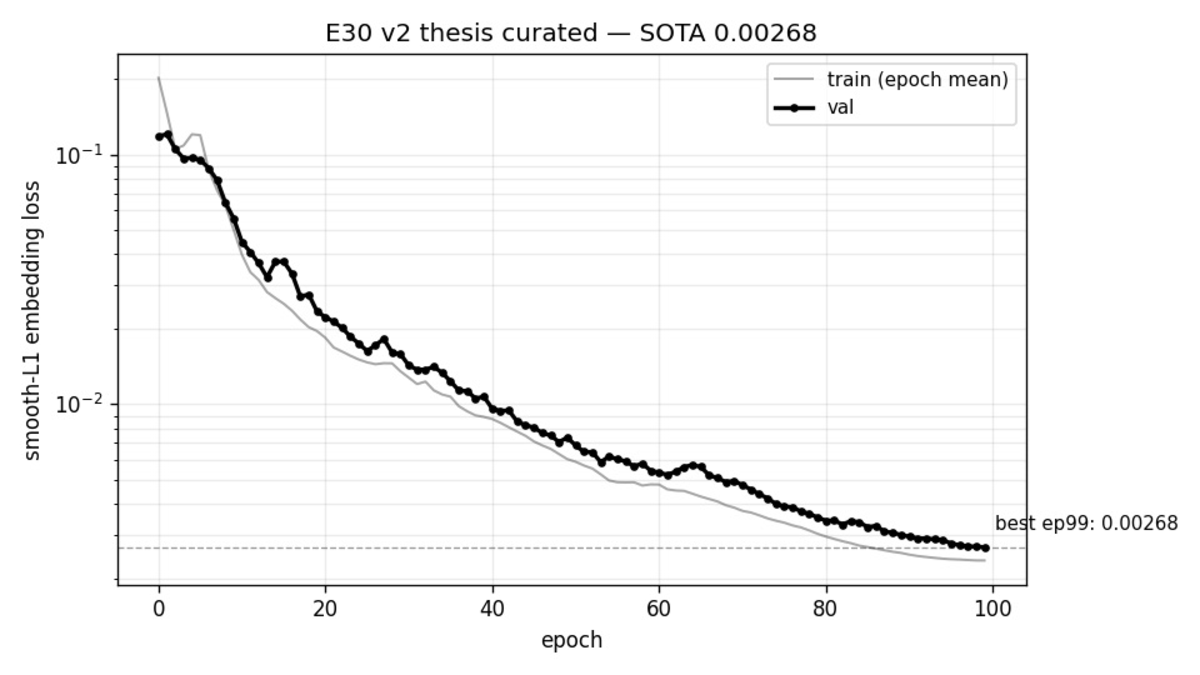
\includegraphics[width=0.75\linewidth]{assets/figures/curves_thesis_run.pdf}
\caption{Validation smooth-$L_{1}$ versus epoch for the E30
thesis run, thirteen training cubes and three validation cubes,
one hundred epochs of two thousand steps each on the 5060\,Ti
CUDA backend.}
\label{fig:curves-thesis-app}
\end{figure}
\FloatBarrier

\section{Best-loss summary}
\label{app:curves-summary}

\begin{table}[htbp]
\centering
\small
\begin{tabular}{lll}
\toprule
Run                              & Best val (smooth-$L_{1}$) & Epoch \\
\midrule
E12 (tube only)                  & $0.04017$ & $42 / 100$ \\
E13 (tube $+$ future)            & $0.01812$ & $92 / 100$ \\
E14 (tube $+$ cross-time)        & $0.01172$ & $91 /  99$ \\
E15 (uniform mix, anchor)        & $0.00530$ & $100/100$ \\
E17 ($\tau = 0.990$)             & $0.00761$ & $101/101$ \\
E18 ($\tau = 0.994$)             & $0.00938$ & $100/100$ \\
E19 ($\tau = 0.998$)             & $0.01107$ & $100/100$ \\
E20 ($\tau = 0.9995$)            & $0.03010$ & $100/100$ \\
E25 (ratio $0.60$)               & $0.00960$ & $99 /100$ \\
E26 (ratio $0.75$, winner)       & $0.00876$ & $99 /100$ \\
E27 (ratio $0.85$)               & $0.01597$ & $99 /100$ \\
E28 (ratio $0.90$, terminated)   & $0.05798$ & $36 /100$ \\
\bottomrule
\end{tabular}
\caption{Summary of best validation loss across the ablations of
Chapter~\ref{ch:experiments}. Values are read from the per-run
\texttt{run.jsonl} artefacts on disk.}
\label{tab:best-losses}
\end{table}

\begin{figure}[htbp]
\centering
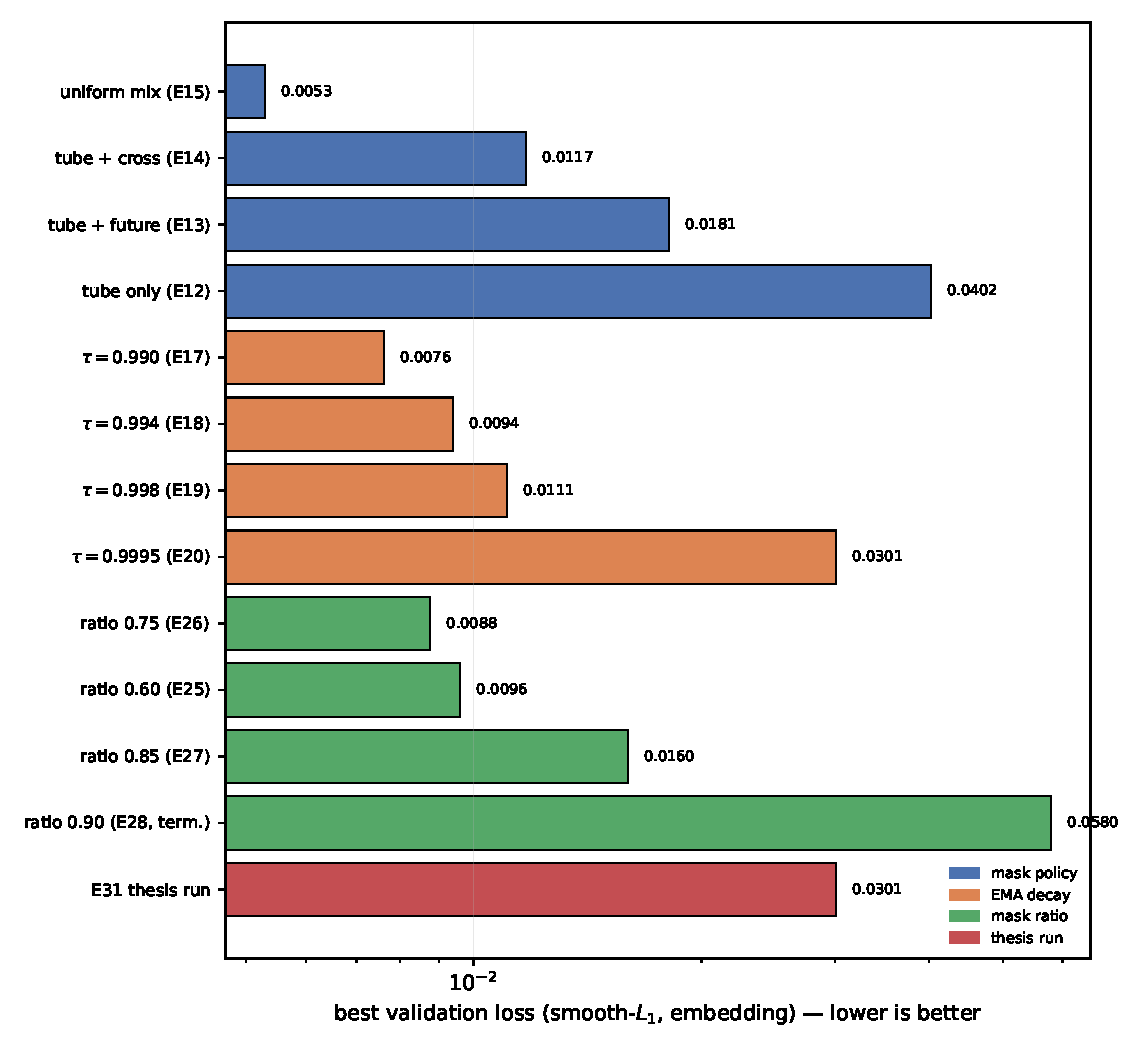
\includegraphics[width=0.92\linewidth]{assets/figures/ablation_summary.pdf}
\caption{Bar chart of the best-loss summary in
Table~\ref{tab:best-losses}. Lower is better.}
\label{fig:ablation-summary-app}
\end{figure}
